%%%%%%%%%%%%%%%%%%%%%%%%%%%%%%%%%%%%%%%%%%%%%%%%%%%%%%%%%%%%%%%%%%%%%%%%%%%%%%%%%
\section{Inleiding}
\emph{Redirected walking} is een techniek waarbij een proefpersoon in een 
virtuele omgeving weergegeven in een head-mounted display kan rondwandelen door 
middel van het vervormen van de route die deze proefpersoon in een fysieke 
omgeving wandelt. Het doel is, door de 1:1 relatie van fysieke beweging en 
virtuele beweging te ontkoppelen, rondwandelen in grotere tot zelfs arbitrair 
grote virtuele ruimtes mogelijk te maken. Ik zal diverse technieken bespreken die
gebruikt worden om deze ontkoppeling teweeg te brengen. Naast de
redirectietechnieken zijn er ook technieken die de immersie verbeteren door
andere zintuigen te betrekken bij het proces.

%%%%%%%%%%%%%%%%%%%%%%%%%%%%%%%%%%%%%%%%%%%%%%%%%%%%%%%%%%%%%%%%%%%%%%%%%%%%%%%%%
\section{Redirectietechnieken (RDTs)}
RDTs zijn technieken waar de fysieke bewegingen van een proefpersoon ontkoppeld
worden van de resulterende virtuele bewegingen. Dit kan bijvoorbeeld gebeuren 
door de snelheid van de proefpersoon in de virtuele omgeving te versnellen of te
vertragen ten opzichte van de snelheid in de fysieke omgeving, of door de
rotaties te vertragen of te versnellen zodat de proefpersoon het tracking gebied
niet verlaat. Ik beschrijf hier kort enkele van deze technieken samen met 
onderzoeken die er over gevoerd zijn.


\subsection{Rotationele vervorming}
Bij rotationele vervorming worden de rotaties van de proefpersoon in de 
virtuele omgeving vertraagd of versneld ten opzichte van de rotaties in de
fysieke omgeving, een voorbeeld hiervan kan men zien in Figuur 
\ref{fig:kohn01-movement}.

\begin{figure}[h!]
    \centering
    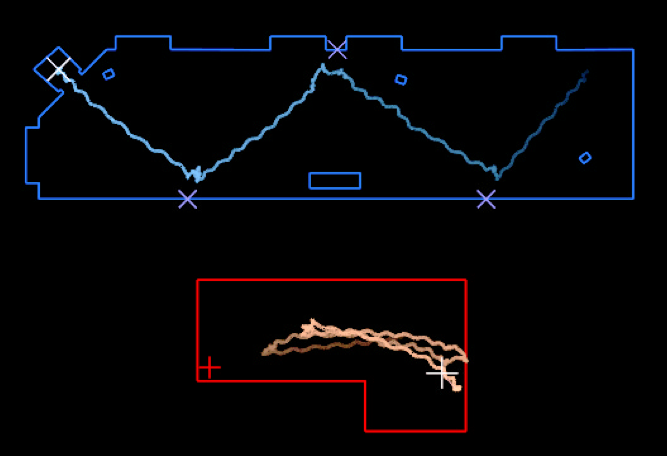
\includegraphics[width=0.7\textwidth]{kohn01-movement}
    \caption{Vergelijking van de beweging van de proefpersoon in de virtuele
    omgeving (blauw) en de overeenkomstige beweging in de fysieke omgeving 
    (rood).\cite{kohn01}}
    \label{fig:kohn01-movement}
\end{figure}

Deze techniek is al in diverse papers onderzocht:

In een onderzoek gevoerd door Razzaque et. al., 2001 \cite{kohn01} werden 
proefpersonen gevraagd om een virtuele brandoefening uit te voeren. In de 
opstelling voor dit onderzoek waren er in het fysieke labo twee knoppen geplaatst
op dezelfde afstand als in de virtuele omgeving. In de virtuele omgeving waren er
echter 4 knoppen met telkens een hoek van 90 graden er tussen, deze opstelling is
in bovenaanzicht getoond in Figuur \ref{fig:kohn01-movement}. In dit onderzoek
werd op enkele verschillende manieren rotationele vervorming ingevoegd:

Als de proefpersoon stilstaat werd er een kleine hoeveelheid ``drift'' 
toegevoegd, de camera in de virtuele omgeving draaide automatisch zeer traag in 
de omgekeerde richting van waar men de proefpersoon in de fysieke omgeving heen 
wilde naar laten kijken. Het bleek dat de proefpersoon hierdoor automatisch in
die richting ging draaien om het beeld stil te houden. De rotaties van de
proefpersoon werden ook overdreven, of juist gedempt, om de proefpersoon in de
fysieke omgeving in de juiste richting te laten wandelen.

Naast deze vervormingen indien de testpersoon in stilstand was, was het ook
mogelijk om een schijnbaar rechte lijn in de virtuele omgeving overeen te laten
komen met een curve. Dit effect werd bekomen door het pad in de virtuele omgeving
een bepaalde hoeveelheid te buigen, proportioneel met de lineaire snelheid van
de proefpersoon in de fysieke omgeving.

<<<<<<< HEAD
% CONTINUE
=======
\todo{continue here}
>>>>>>> Begin reworking litstudy.

Deze gegevens werden dan gebruikt om de proefpersoon in de richting van de 
volgende knop te sturen zodat de proefpersoon voor een fysieke knop stond als dit 
ook het geval was in de virtuele omgeving.

Dit onderzoek vereist een voorberekend pad en een minimale deviatie van dit pad 
door de proefpersoon voor een optimale ervaring. In Engel et. al., 2008 
\cite{engel08} wordt een techniek voorgesteld om deze rotationele vervorming 
dynamisch te bepalen.

Dit werd gedaan door het dynamische-rotatie probleem te reduceren tot een 
optimisatie probleem, welke in de AI gemeenschap reeds bekend zijn.

Dit algoritme maakte het mogelijk om optimale rotationele vervormingen te 
berekenen maar vereist in ieder geval een gedeeltelijke kennis over het te volgen
virtuele pad.

In een ander onderzoek in Neth et. al., 2012 \cite{neth12} werd verder 
onderzocht wat de precieze relatie tussen bewegingssnelheid en maximaal 
acceptabele rotationele vervorming is.

Uit dit onderzoek bleek dat tragere snelheden grotere vervormingen toelaten, maar
dat deze relatie niet lineair is.

Aangezien mensen over het algemeen trager wandelen in virtuele omgevingen
\cite{mohler07}, kan men dit toepassen in redirected walking.

In een tweede experiment \cite{neth12} werd onderzocht of deze bevindingen
effectief konden gebruikt worden dynamische schalering van vervorming toe te
passen in een rijke virtuele omgeving. Er werd hier onderzocht of er een
significant verschil is tussen de effectiviteit van statische rotationele
vervorming versus dynamische rotationele vervorming.

Naast de technieken van Razzaque et. al., 2001 \cite{kohn01} om rotationele
vervorming in te voegen met een constant, een statisch en een dynamisch 
component, werd er ook gebruik gemaakt van versterking van de effecten nabij de 
randen van de fysieke omgeving, om het verlaten van het tracking gebied te 
vermijden.

Er werd gemeten wat de mediaanafstand is die een proefpersoon kan wandelen in 
een grote virtuele omgeving voor de proefpersoon moet geforceerd 
geherori\"enteeerd worden richting het centrum van de fysieke omgeving om het 
verlaten van het tracking gebied te voorkomen.

Uit dit experiment is gebleken dat er een positief significant verschil is tussen
de mediaan gewandelde afstand bij dynamische vervorming versus statische
vervorming zonder een significante verhoging in simulatorziekte.

Uit al deze onderzoeken blijkt dat er een trade-off is tussen een virtuele 
omgeving met een ongekend pad\cite{neth12} versus een betere immersie wegens 
minder onderbrekingen\cite{engel08,kohn01}. 

Alle vorige studies behandelden rotationele vervorming in beweging, dus over 
curves. Het is echter ook mogelijk om rotationele vervorming in stilstand te
hebben.

In \cite{steinicke09} werd bepaald dat in dit specifieke geval compressies tot
77\% acceptabel zijn voor de proefpersoon het merkt.

Rotationele vervorming vormt de basis van redirected walking, gegeven een
voldoende grote ruimte kan deze techniek toegepast worden om elke virtuele
omgeving te doorlopen.


\subsection{Translationele vervorming}
Naast rotationele vervorming is het ook mogelijk om de lineaire snelheid van een
proefpersoon te vervormen daar onderzoek heeft aangetoond dat proefpersonen in 
virtuele omgevingen afstand \cite{loomis03}, snelheid \cite{banton05} en 
afgelegde afstand \cite{frenz07} onderschatten.

In Steinicke et. al., 2009 \cite{steinicke09} werd er een experiment uitgevoerd 
om onder andere te bepalen wat de maximaal acceptabele translationele vervorming 
is voor een gegeven snelheid.

Er werd bepaald dat de vervorming merkbaar is bij een versnelling tussen 20\% en
60\% met een ideale waarde van ongeveer 20\%.

Translationele vervorming vormt samen met rotationele vervorming een ideale basis 
om realistische redirected walking toe te passen, maar toch de benodigde fysieke 
ruimte tot een minimum te houden.


\subsection{Change blindness}
\todo{MEER}
Een alternatieve methode, zonder ontkoppeling van de 1:1 relatie tussen fysieke 
en virtuele locatie is het gebruik maken van change blindness.

In Suma et. al., 2011 \cite{suma11} werd er getest of veranderingen in de 
virtuele omgeving voor de proefpersonen merkbaar waren. In een virtuele omgeving 
werd de locatie van de deur in een kamer veranderd zodra de proefpersoon weg 
keek.

Uit dit experiment is gebleken dat, in zulke omstandigheden, veranderingen in de
virtuele omgeving voor zowel ervaren als na\"ieve proefpersonen onmerkbaar zijn.


%%%%%%%%%%%%%%%%%%%%%%%%%%%%%%%%%%%%%%%%%%%%%%%%%%%%%%%%%%%%%%%%%%%%%%%%%%%%%%%%%
\section{Reori\"entatietechnieken (ROTs)}
ROTs zijn technieken om te voorkomen dat de proefpersoon het fysiek trackbare 
gebied verlaat.

In tegenstelling tot RDTs zijn deze technieken niet noodzakelijk onmerkbaar, ik
beschrijf er hier enkele.


\subsection{Verbale commandos}
In het onderzoek van Razzaque et. al., 2001 \cite{kohn01} werd, indien de
proefpersoon dreigde het tracking gebied te verlaten, de proefpersoon met verbale
commando's gevraagd stil te staan en heen en weer te kijken om de proefpersoon in
de fysieke omgeving terug in de juiste richting te laten kijken.

Er werd in een andere studie van Peck et. al., 2009 \cite{peck09} echter bevonden 
dat verbale commando's niet de beste optie zijn voor redirectietechnieken, en dat
afleidingen betere resultaten geven.


\subsection{Visuele commandos}
In het onderzoek van Neth et. al., 2012 \cite{neth12} werd onder andere gebruik 
gemaakt van een stopteken. Als dit werd getoond werd de hele virtuele wereld stil 
gelegd. Er werd op voorhand aan de proefpersoon gevraagd rond te draaien tot het 
stopteken verdwijnt indien het getoond werd.

Hoewel dit een zeer intrusieve methode is, is ze zeer effectief om het verlaten
van het tracking gebied te voorkomen.


\subsection{Afleiders}
Bovenstaande ROTs zijn allemaal erg intrusief, daarom is er een derde categorie
van ROTs die tracht zo onopvallend mogelijk te zijn.

Dit is de categorie van de afleidingen, zoals andere ``personen'' in de virtuele
omgeving\cite{neth12}, om de proefpersoon subtiel in de juiste richting te 
leiden.

In Peck et. al., 2009 \cite{peck09} wordt er onder andere gebruik gemaakt van een 
te volgen object (een vlinder) om de proefpersoon de illusie te geven dat hij 
\mbox{360\textdegree} heeft gedraaid terwijl hij eigenlijk maar 180\textdegree{}
heeft gedraaid. Hieruit bleek dat proefpersonen minder het gevoel hadden dat de
wereld versneld draaide met een afleiding dan bij andere technieken.


%%%%%%%%%%%%%%%%%%%%%%%%%%%%%%%%%%%%%%%%%%%%%%%%%%%%%%%%%%%%%%%%%%%%%%%%%%%%%%%%%
\section{Andere zintuigen}
Hoewel visie voor redirected walking het belangrijkst is, omdat bij conflicten
tussen het proprioceptieve en het vestibulaire systeem en visie, visie vaak dit
conflict wint\cite{berthoz02,dichgans78,bruder08}, zijn de andere zintuigen toch
belangrijk om immersie te verkrijgen. 

Als men in een virtuele omgevingen geluid realistisch kan positioneel
reproduceren helpt dit bijvoorbeeld de immersie enorm\cite{lackner77}, maar zelf
het maskeren van geluid van in de fysieke wereld met bijvoorbeeld ruis kan
helpen\cite{usoh99}.

In Engel et. al., 2008\cite{engel08} wordt ook opgemerkt dat de hoeveelheid 
omgevingslicht en omgevingsgeluid dat binnensijpelt een merkbare negatieve 
invloed heeft op de effectiviteit van redirectietechnieken.

Naast audio is het ook mogelijk om de immersie te verhogen met proxy-objecten in
de fysieke omgeving die overeen komen met objecten in de virtuele 
omgeving\cite{steinicke09}.


%%%%%%%%%%%%%%%%%%%%%%%%%%%%%%%%%%%%%%%%%%%%%%%%%%%%%%%%%%%%%%%%%%%%%%%%%%%%%%%%%
\section{Inherente zwaktes}
Hoewel redirected een realistische en immersieve omgeving kan cre\"eren zijn er
toch enkele inherente zwaktes waar op zich niet omheen kan gewerkt worden.

Zo is het bijvoorbeeld onmogelijk om arbitraire fysieke collisie overeen te laten
komen met collisie in de virtuele omgeving tenzij het labo expliciet voor die
virtuele omgeving is gebouwd.

Een ander voorbeeld is dat het onmogelijk is om heuvels of ander ruw terrein te
hebben in de virtuele omgeving zonder immersie te breken.

Desondanks deze behoorlijke beperkingen heeft redirected walking toch veel
potenti\"ele toepassingen zoals virtuele rondleidingen.


%%%%%%%%%%%%%%%%%%%%%%%%%%%%%%%%%%%%%%%%%%%%%%%%%%%%%%%%%%%%%%%%%%%%%%%%%%%%%%%%%
\section{Positionele tracking \& Head-mounted diplays (HMDs)}
Naast het software aspect van redirected walking is er ook het hardware aspect
van het positioneel tracken en het head-mounted display.

Er zijn twee grote categorie\"en van head trackers. Inwaartse tracking, waar de
proefpersoon door \'e\'en of meer camera's in de omgeving wordt getrackt. En
uitwaartse tracking, waar een camera aan de proefpersoon hangt en deze de
omgeving trackt.

In het algemeen wordt bij redirected walking gebruik gemaakt van inwaartse 
tracking\cite{bruder08,engel08,steinicke09,kohn01,neth12,ward92}. Er zijn ook 
commerci\"ele uitwaartse tracking systemen die gebruikt worden in redirected
walking onderzoeken\cite{peck09,suma11}. Verder is er nog actief onderzoek naar
betere uitwaartse tracking systemen\cite{maesen13}.

Voor HMDs is het ideaal om een zo hoog mogelijke field of view te hebben, dit
lijkt geen groot effect te hebben op de prevalentie van 
simulatieziekte\cite{arthur00} maar verhoogt de performantie en immersie
drastisch\cite{arthur00}.

Traditioneel waren HMDs met hoge field of view zeer duur en niet beschikbaar voor
consumenten, maar tegenwoordig zijn er enkele betaalbare HMDs beschikbaar met een
redelijk hoge field of view, zoals de Oculus Rift DK1 (110\textdegree{} 
diagonaal).